\documentclass[a4paper]{jpconf}
\usepackage{graphicx}
\usepackage{color}
\begin{document}
\title{Event processing time prediction at the CMS experiment of the Large Hadron Collider}

\author{Samir Cury$^1$, Oliver Gutsche$^2$ and Dorian Kcira$^3$}

\address{$^{1,3}$ California Institute of Technology}
\address{$^2$ Fermi National Accelerator Laboratory}

\ead{$^1$ samir@hep.caltech.edu, $^2$ gutsche@fnal.gov, $^3$ dkcira@caltech.edu}

\begin{abstract}
  The physics event reconstruction is one of the biggest challenges for the computing of the LHC experiments.
  %
  Among the different tasks that computing systems of the CMS experiment performs, the reconstruction takes most of the available CPU resources. The reconstruction time of single collisions varies according to event complexity. Measurements were done in order to determine this correlation quantitatively, creating means to predict it based on the data-taking conditions of the input samples.
  %
  Currently the data processing system splits tasks in groups with the same number of collisions and does not account for variations in the processing time. These variations can be large and can lead to a considerable increase in the time it takes for CMS workflows to finish.
%
The goal of this study was to use estimates on processing time to more efficiently split the workflow into jobs. By considering the CPU time needed for each job the spread of the job-length distribution in a workflow is reduced.
\end{abstract}

\section{Introduction}

The main goal of this study is to find the factors from data-taking with most influence the processing time of the resulting saved collision data (also called ``events''). After quantifying the relation between these factor and the event processing times, systematic deviations are studied as a result of the data-taking parameters and the reduction of those systematic effects is addressed.

It is expected that one of the main factors that influences event processing time is the charged particle track multiplicity of those events. Measurements are presented below of the relation between the two and a method is developed for predicting the processing time of future data in the same luminosity range.

\section{Accelerator and collisions}

\subsection{Charged particle track multiplicity}

\begin{figure}[ht]
  \begin{center}
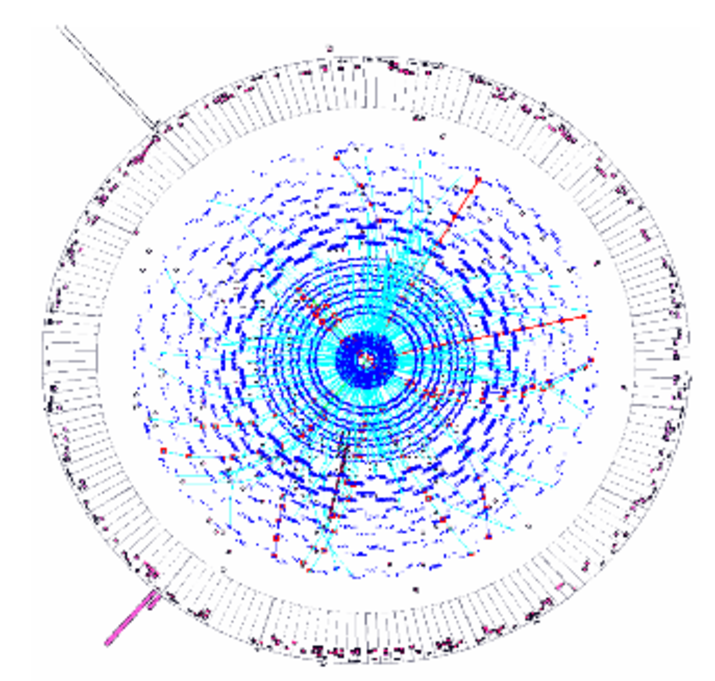
\includegraphics[width=0.4\textwidth]{1.pdf}
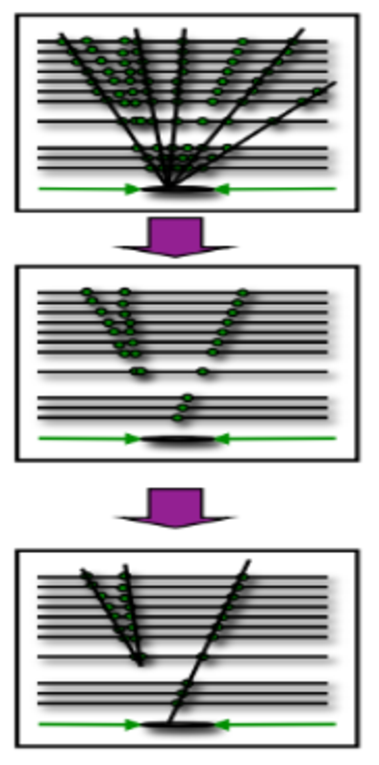
\includegraphics[height=0.55\textwidth,angle=90]{2.pdf}
\caption{\label{fig1} Visualization of a collision with several charged tracks in the CMS detector (left). Schematic representation of the steps for the reconstruction and disambiguation of tracks out of many different hits in the CMS tracking system (right).}
  \end{center}
\vspace{-8mm}
\end{figure}

The complexity of track reconstruction is to a large extent due to the large number of charged particle tracks from the collisions as well as the overlap among these collisions. Iterations become thus necessary in order  not only to fit hits in the tracking detectors but also to disentangle the different possibilities resulting from the large combinatorics (see figure~\ref{fig1} on page \pageref{fig1}). The number of hits used for track reconstruction depends strongly on instantaneous luminosity and the number of collisions that happen simultaneously per beam bunch crossing (pile-up interactions). Pile-up itself is a function of the accelerator running conditions and instantaneous luminosity. This study focuses, therefore, on instantaneous luminosity.


\subsection{Instantaneous luminosity}

2012 was the most challenging year for the LHC Run1 data-taking (2010 to the first quarter of 2013). The LHC operational energy was 8~TeV. Record instantaneous luminosity values of the collisions were achieved from the LHC and the resulting collisons measured in the CMS detector. This, on its turn, translates into large track multiplicities and increasing the number of pile-up (PU) interactions per bunch-crossing.

\begin{figure}[ht]
  \begin{center}
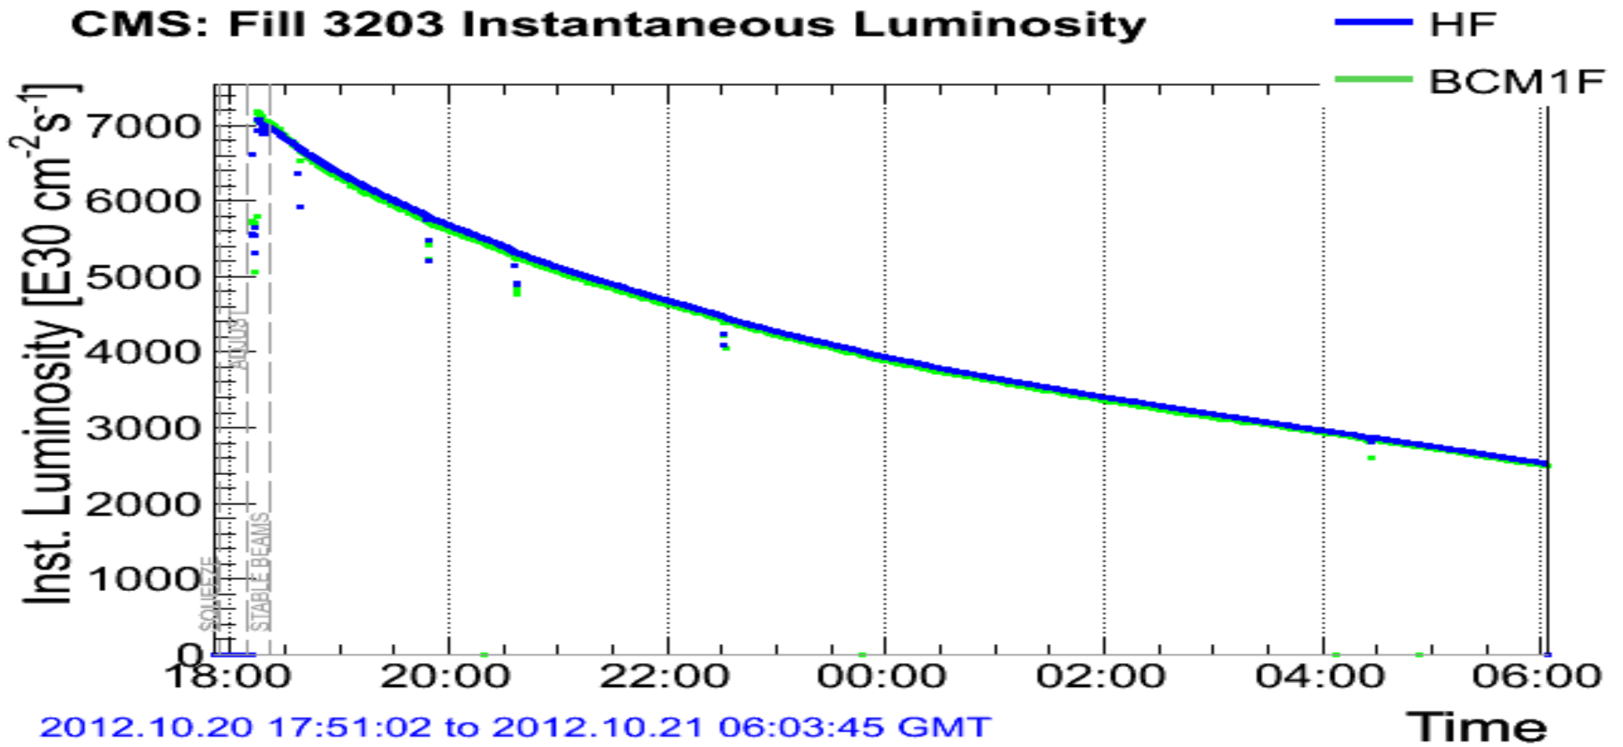
\includegraphics[width=0.32\textwidth,height=0.34\textwidth]{6.pdf}
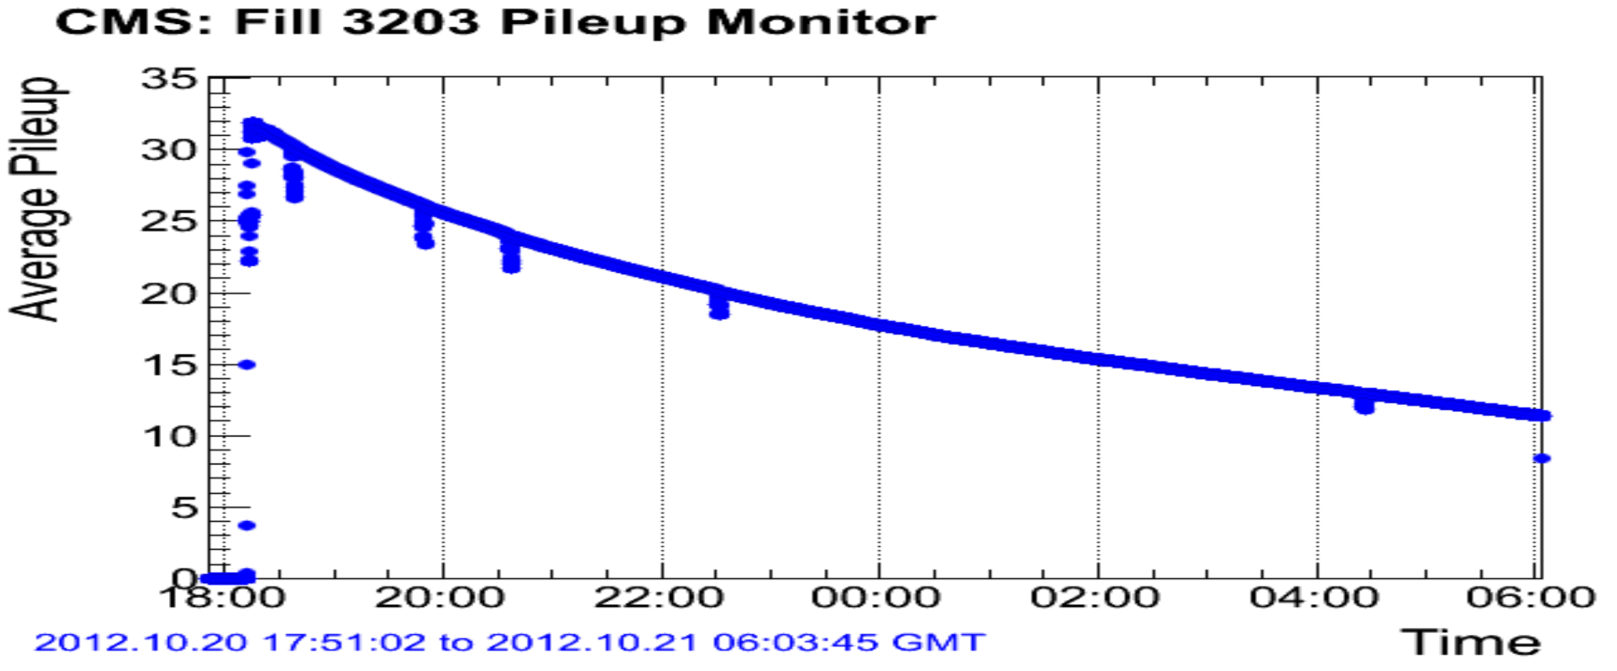
\includegraphics[width=0.32\textwidth,height=0.34\textwidth]{5.pdf}
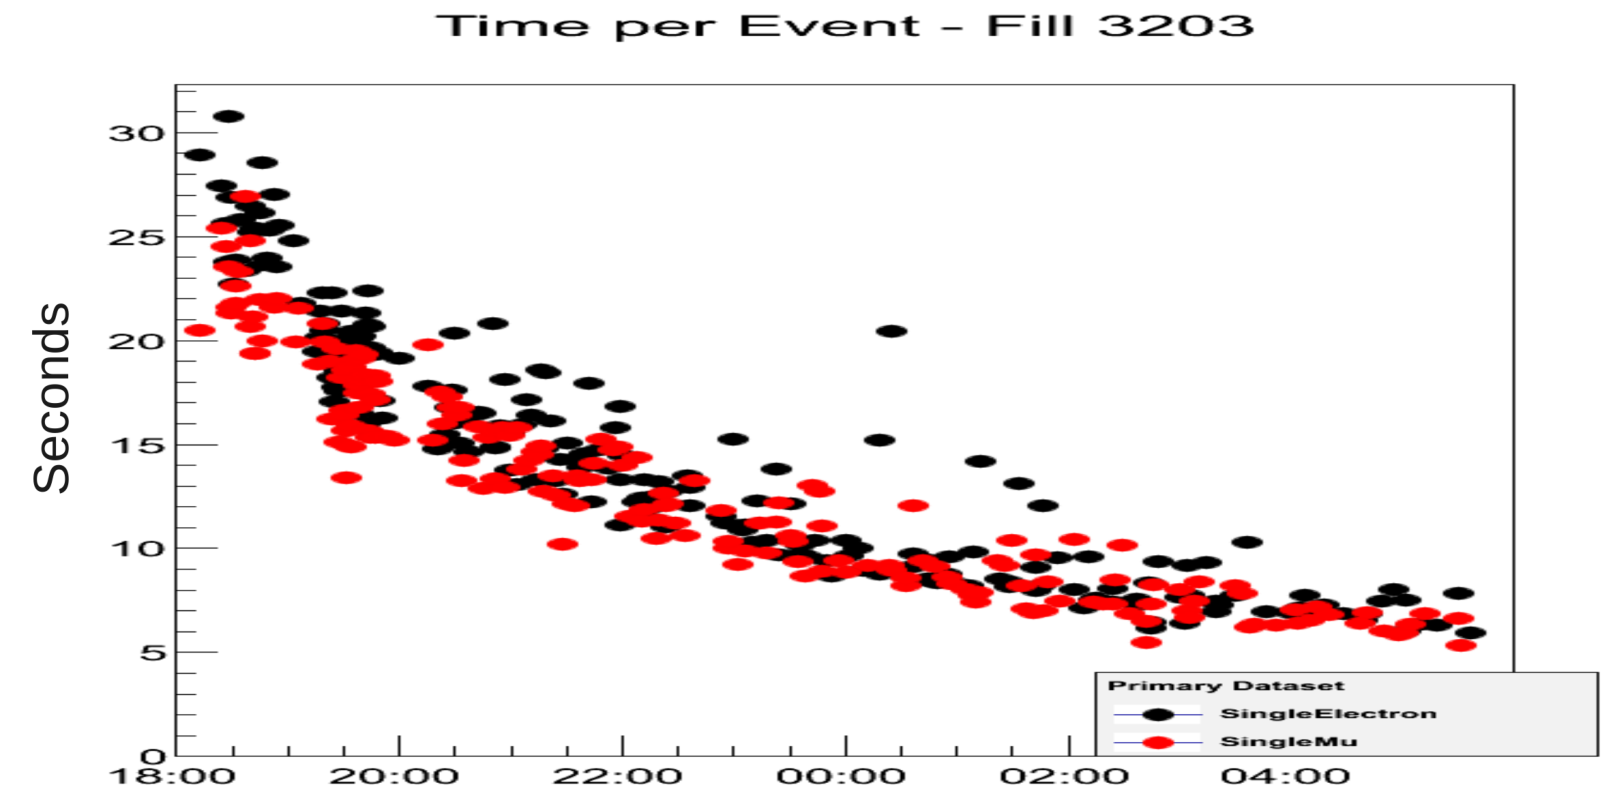
\includegraphics[width=0.32\textwidth,height=0.34\textwidth]{7.pdf}
\caption{\label{fig2} Instantaneous luminosity (left), pile-up curve (middle), and event processing time (right) as a function of the passing time within a data-taking run at the CMS experiment.}
  \end{center}
\vspace{-7mm}
\end{figure}

In a typical data-taking run, the instantaneous luminosity ranges from 7200$ \cdot 10^{30}$cm$^{-2}$s$^{-1}$ at the beginning of the fill to 2500$ \cdot 10^{30}$cm$^{-2}$s$^{-1}$ at the end of the same fill.  This results in a number of PU interactions of about 34 at the beginning of the fill and about 12 at its end. figure~\ref{fig2} on page \pageref{fig2} shows the instantaneous luminosity (left), the pile-up curve (middle) as well as the processing time of events (right) as a function of time during a data-taking run. The proportionality between the three quantities can be observed.




\begin{figure}[ht]
  \begin{center}
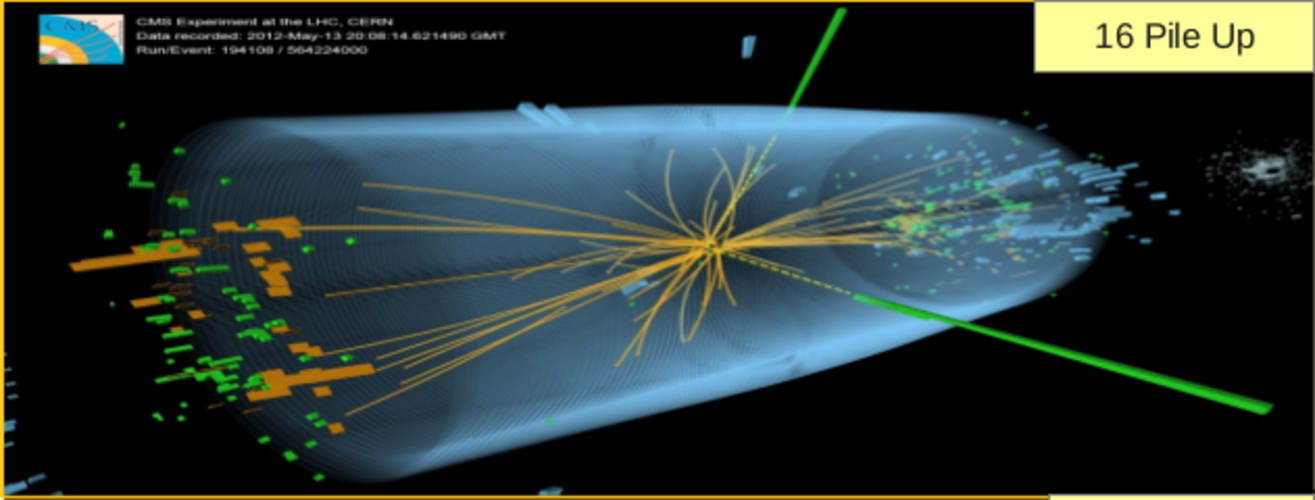
\includegraphics[width=0.45\textwidth,height=0.33\textwidth]{3.pdf}
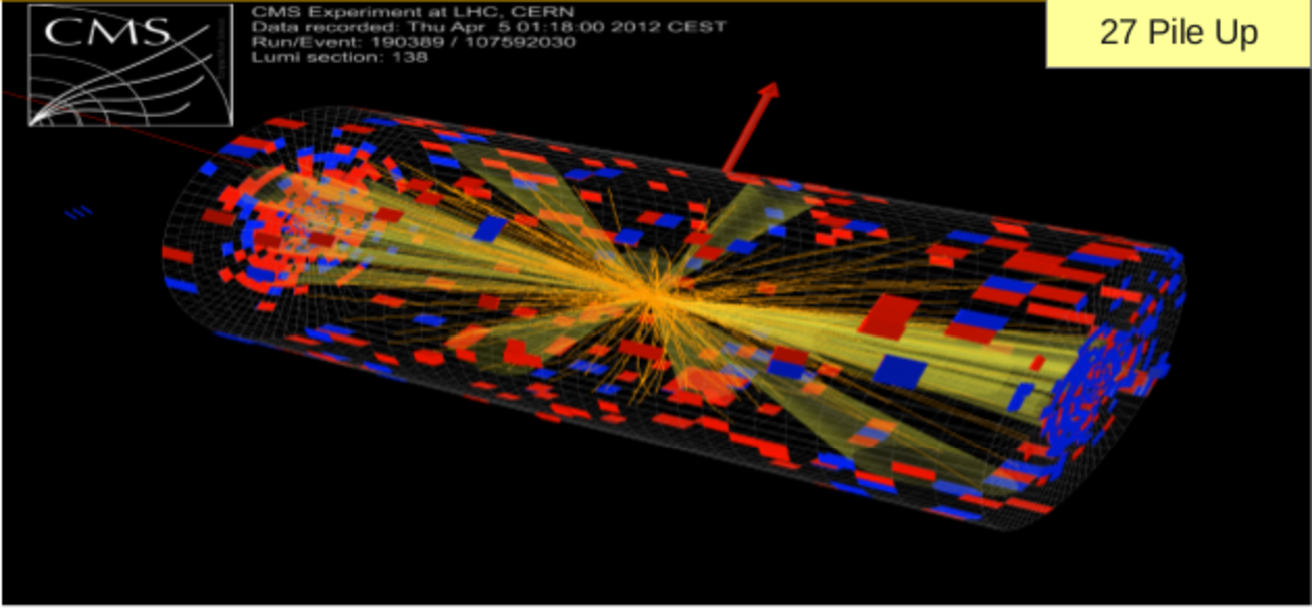
\includegraphics[width=0.45\textwidth,height=0.33\textwidth]{4.pdf}
\caption{\label{fig3} Visualization of events with charged tracks in the CMS detector for the low-luminosity case (left) and the high-luminosity one (right).}
  \end{center}
\vspace{-8mm}
\end{figure}

Figure~\ref{fig3} on page \pageref{fig3} shows event displays of the charged particle tracks in the CMS detector coming out of LHC collisions. Two cases are distinguished, the sparse low-luminosity case (left), with lower number of tracks (16 PU events/bunch crossing), and the dense high-luminosity case (right), with large number of tracks (27 PU/bunch crossing).



\section{Measurements of event processing times}

\subsection{Performance curves}

The computer performance varies significantly according to the type of physics of the events being processed. Different physics signatures naturally produce more, or less tracks. In this study, measurements on existing processed data are used to estimate processing time of future LHC data. One important factor to consider in the estimate are systematic shifts in the measurements caused by the heterogeneity of the processing farms. Different CPU models will result in different processing time for the same collision type. Our measurements have been done over different CPU models so we believe that the resulting average is a representative value that will be the most useful as an estimate for the CMS central operations.

\begin{figure}[ht]
  \begin{center}
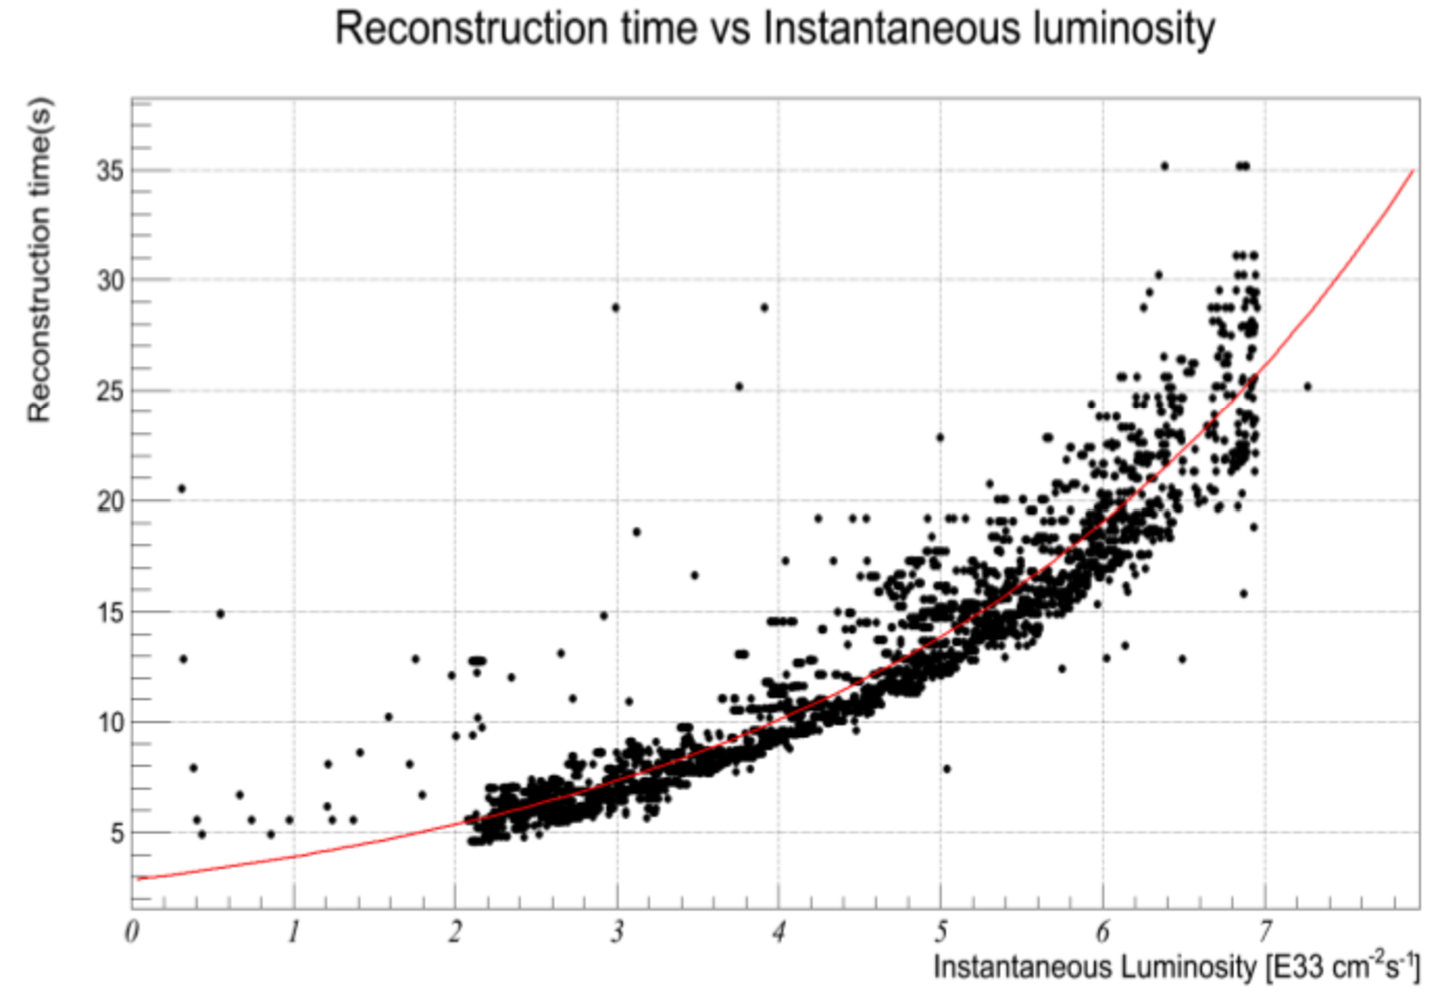
\includegraphics[width=0.32\textwidth,height=0.34\textwidth]{8.pdf}
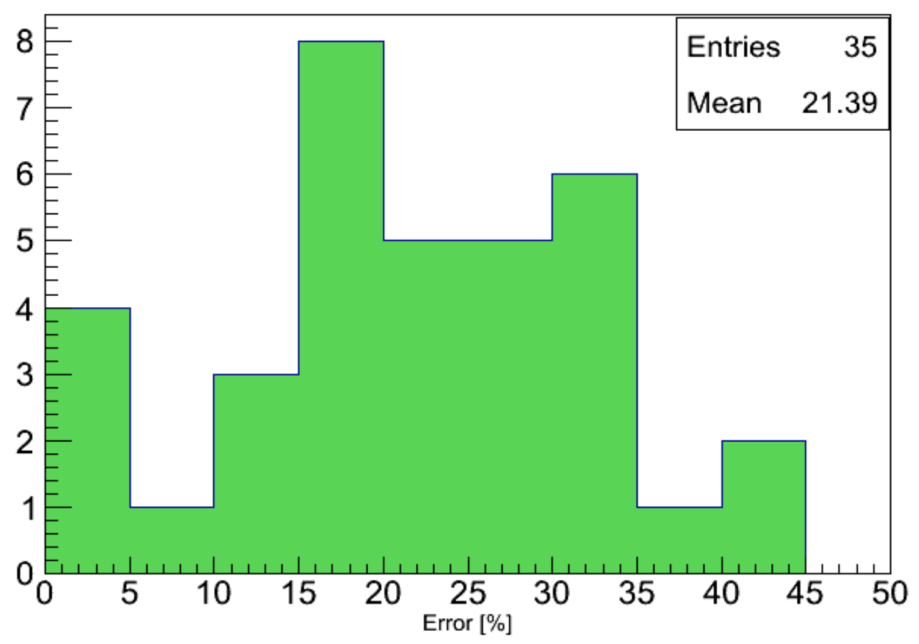
\includegraphics[width=0.32\textwidth,height=0.34\textwidth]{9.pdf}
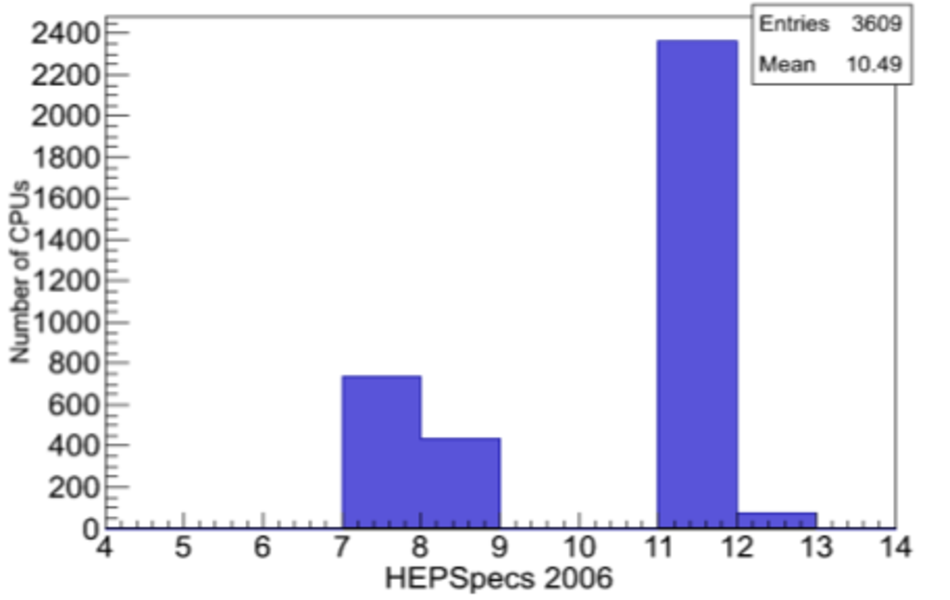
\includegraphics[width=0.32\textwidth,height=0.34\textwidth]{10.pdf}
\caption{\label{fig4} Measurement of the CMSSW performance with respect to event reconstruction time (left). Spread introduced in the reconstruction time by CPU speed fluctuations (middle). Histogram of number of cores in a reconstruction farm in bins of HEPSpec06 values (right).}
  \end{center}
\vspace{-6mm}
\end{figure}


figure~\ref{fig4} on page \pageref{fig4} (left) shows a measurement of the CMS software (CMSSW) performance for a given software release and type of events (primary dataset), in this particular case events with at least one isolated muon (so-called Single Muon). 


\subsection{Systematic errors}

Measurements were done on 35 PromptReco workflows to observe how close to the real value our estimation gets. The error introduced by the CPU speed fluctuation in the Tier~0 farm can be up to 37.75\%. This comes from the difference of HEPSpecs 2006 (benchmark unit) between the fastest and slowest CPU models used.  The results are shown in figure~\ref{fig4} on page \pageref{fig4} (middle).  The green histogram shows the distribution of error values for all workflows. In figure~\ref{fig4} on page \pageref{fig4} (right) the blue is a histogram of the number of cores in the farm per HS06 values, showing how they contribute to the error. %In the table below, some specific measurements, from smaller to bigger error.


\section{Improvements to monitoring and job splitting}

\subsection{Monitoring}

The job-splitting algorithm uses performance information collected at the end of each workflow run by the CMS workflow-management agents (WMAgents).  This information is reported to a specific service maintained by the CMS Dashboard and is used from the data service for automated systems. It is also used by CMS members through a web interface in order to visualize performance curves or average processing times per release and dataset. A performance curve from the CMS Dashboard is shown in figure~\ref{fig5} on page \pageref{fig5} (left).  An example of real log messages that demonstrate how the algorithm works is shown in figure~\ref{fig5} on page \pageref{fig5} (right).

\begin{figure}[ht]
  \begin{center}
\begin{minipage}[t]{0.59\textwidth}
\vspace{0pt}\raggedright
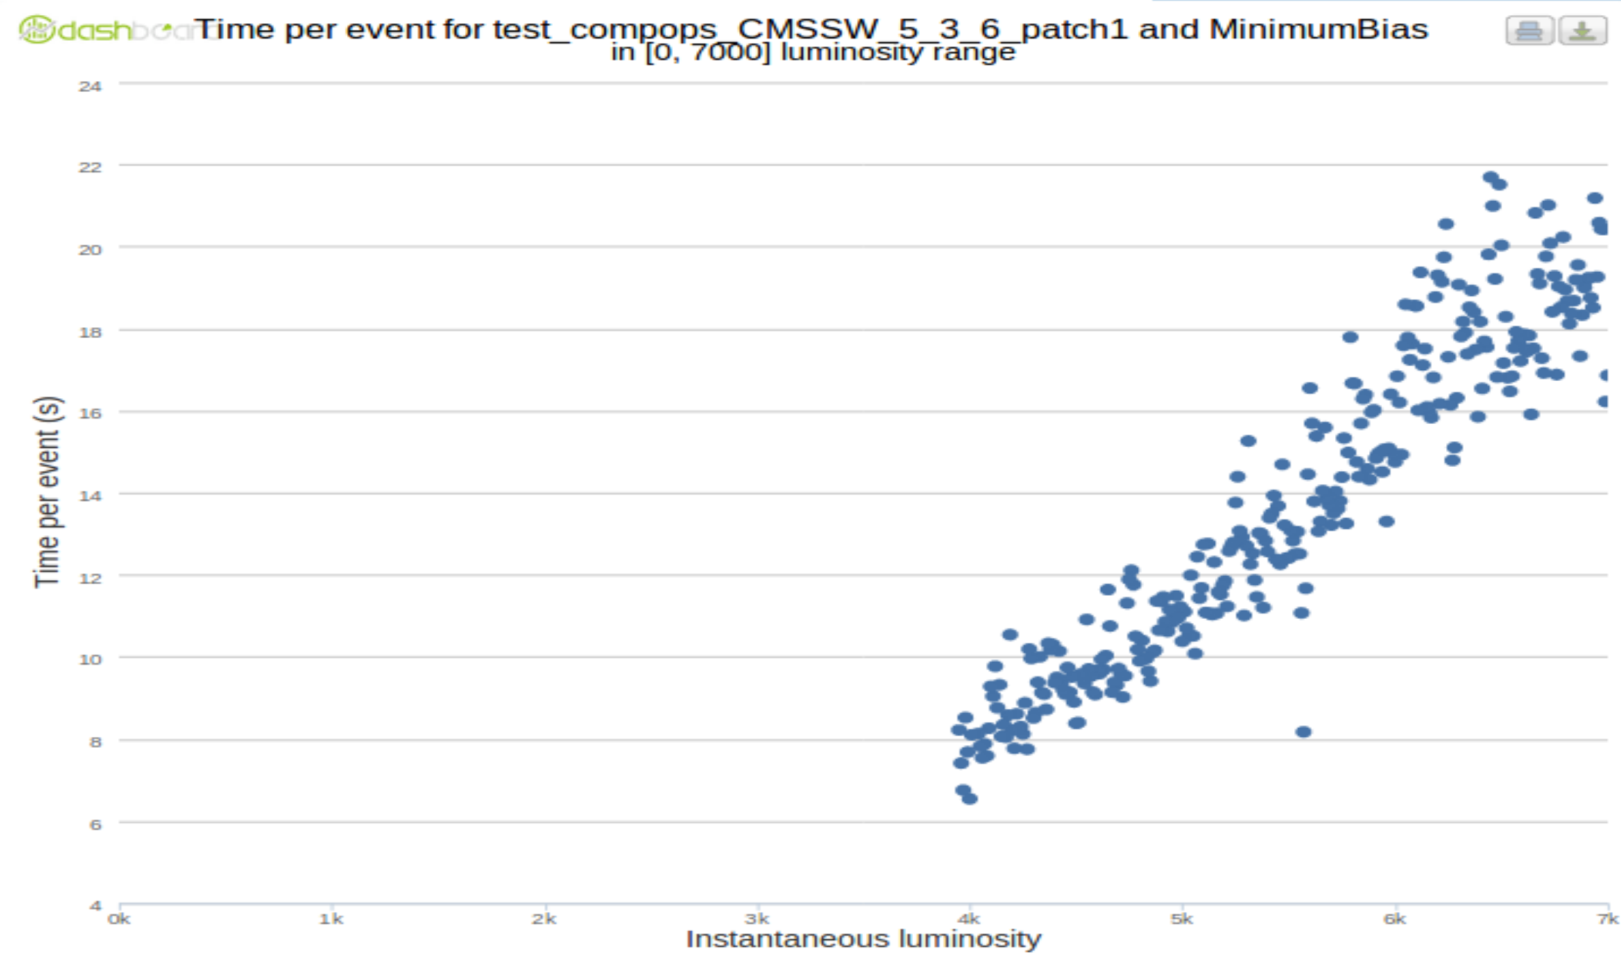
\includegraphics[width=0.99\textwidth,height=0.80\textwidth]{16.pdf}
%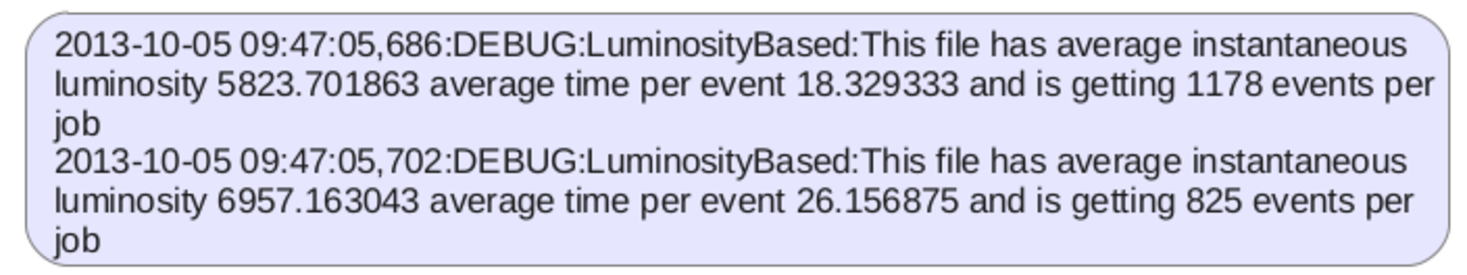
\includegraphics[width=0.40\textwidth,height=0.18\textwidth]{13.pdf}
\end{minipage}
\begin{minipage}[t]{0.40\textwidth}
\vspace{0pt}\raggedright
  \begin{flushleft}
    \textcolor{blue}{
    \small
2013-10-06 09:47:05,045:DEBUG:LuminosityBased:\\
This file has average instantaneous luminosity\\
5202.817391 average time per event 11.358000\\
and is getting 1901 events per job\\
\ \\
2013-10-06 09:47:05,060:DEBUG:LuminosityBased:\\
This file has average instantaneous luminosity
7228.521739 average time per event 27.652917\\
and is getting 781 events per job\\
}
  \end{flushleft}
\end{minipage}
\caption{\label{fig5} CMS DashBoard: Performance curve from reported data (left); An example of real log messages that demonstrate how the algorithm works (right).}
  \end{center}
\vspace{-8mm}
\end{figure}

\subsection{Job splitting}

This study motivated a solution to diminish the long tail effects in CMS data processing. As the relation between instantaneous luminosity and reconstruction time is now well determined, we are able to predict the time-per-event by using the luminosity value from the data. Different CMS web services exist that provide access to this kind of information.  A job-splitting algorithm was developed for the Workload Management Agent that uses this information to estimate a processing time per event. In addition the number of events per processing job is chosen dynamically such that the processing times become more uniform. The ideal processing time per job is approximately 8 hours.


\subsection{Results}

The observed improvements are shown in figure~\ref{fig6} on page \pageref{fig6}. Both the left and right figure are result of the same Reconstruction Workflow. The left figure shows the effect for jobs splitted by the common EventBased algorithm, where the number of events is fixed for all jobs. The second figure shows the case where the splitting is done dynamically by the algorithm LuminosityBased algorithm, described above. A considerably narrower distribution is observed, as expected. This is a result of the job execution time becoming more uniform in the workflows. The algorithm will fall back to the EventBased method for the case where the performance information is not yet available.  The improvements shown here are expected to be even larger in future production systems as the performance information gathered is expected to increase.

\begin{figure}[ht]
  \begin{center}
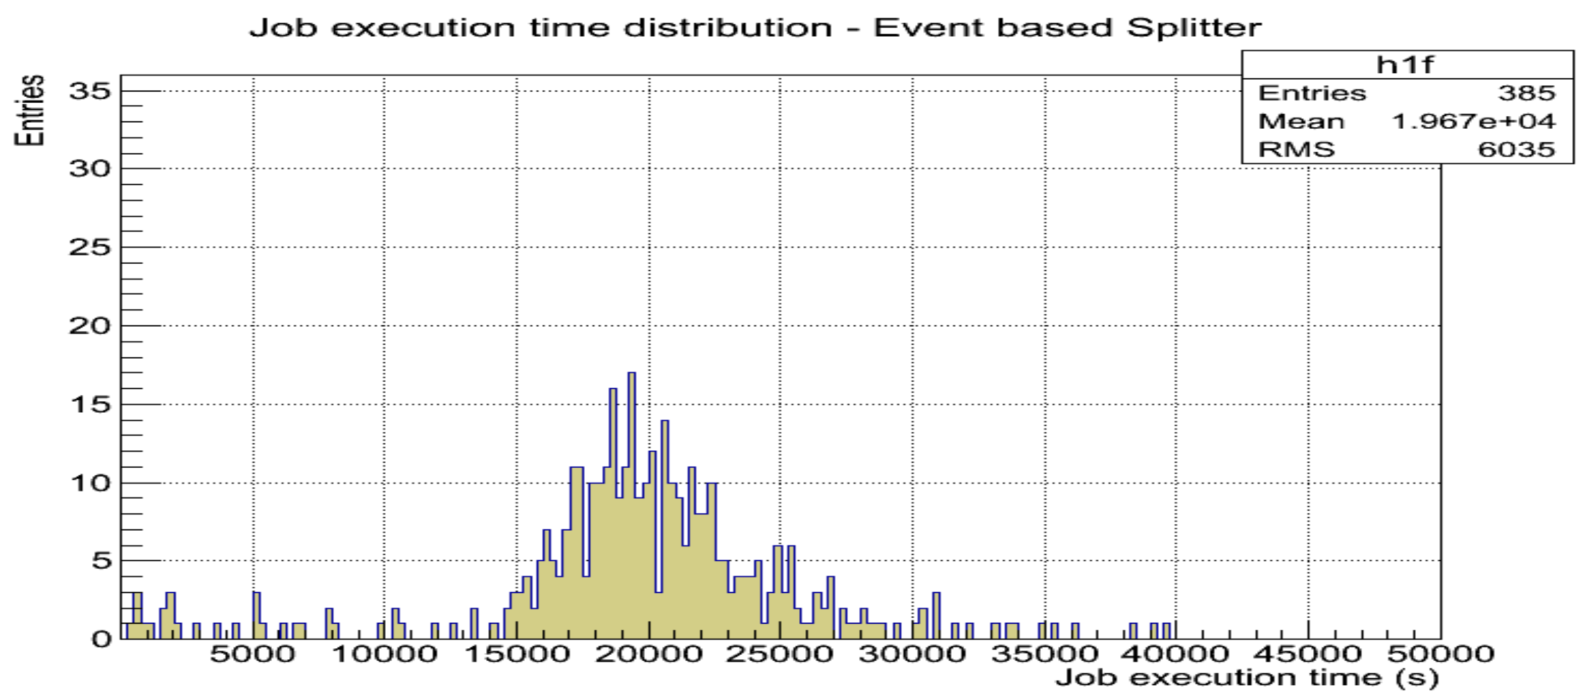
\includegraphics[width=0.47\textwidth,height=0.47\textwidth]{17.pdf}
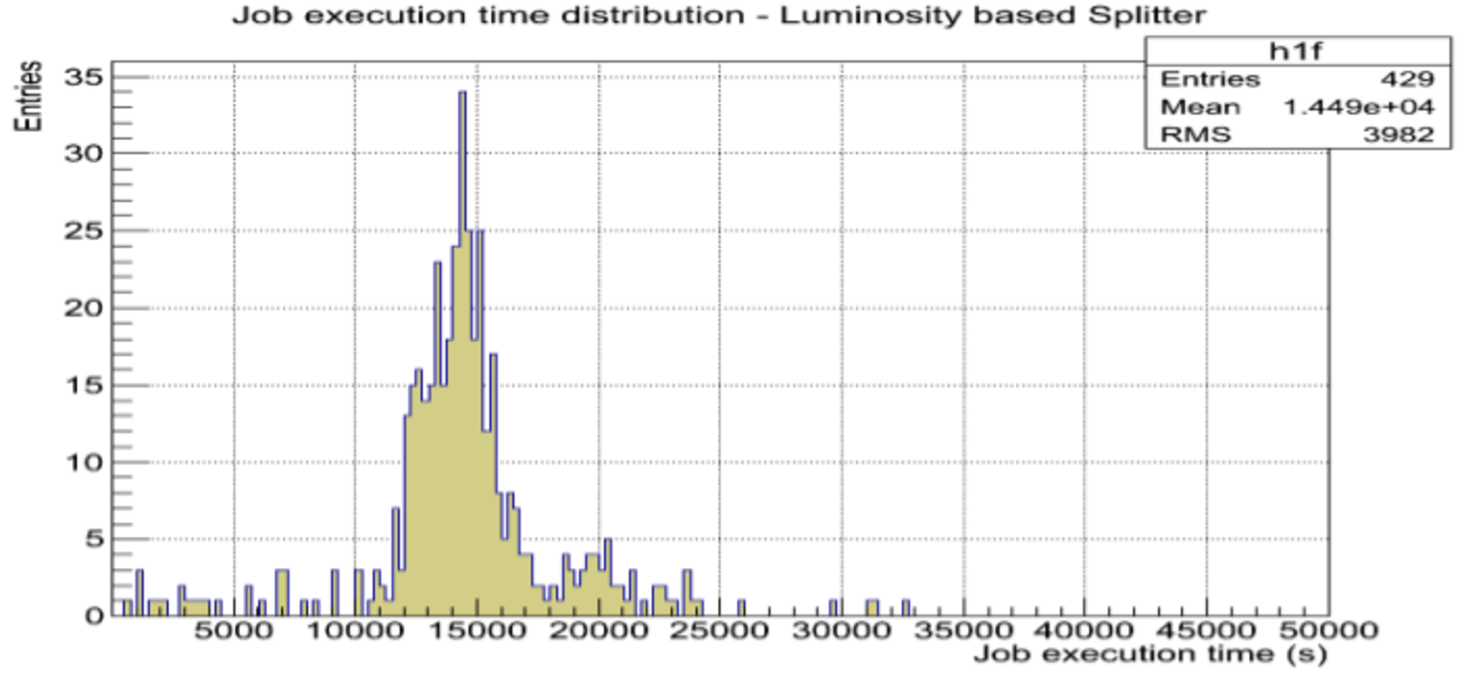
\includegraphics[width=0.47\textwidth,height=0.47\textwidth]{18.pdf}
\caption{\label{fig6} CMS DashBoard: Performance curve from reported data (left); An example of real log messages that demonstrate how the algorithm works (right).}
  \end{center}
\vspace{-8mm}
\end{figure}


\section{Conclusions}

This initial study shows that it is feasible to estimate the time-per-event behavior for reconstruction workflows of CMS. It was observed that heterogeneous computing farms introduce considerable systematic variations into the workflows. This behavior can be taken into account and corrected for. We demonstrated how this information can be used in order to reduce the data processing tails, which have been until now a problem for CMS central production, impacting time-critical prompt-reconstruction workflows in the CMS Tier~0. Furthermore, a job splitting algorithm has been developed that uses performance data dynamically according to the data-taking conditions for the input samples.

\section*{Acknowledgements}

CMS Tier~0 Team, CMS Workload Management Development Team, WLCG DashBoard Team, UERJ Department of High Energy Physics, US-CMS group at the California Institute of Technology, US-CMS group at the Fermi National Accelerator Laboratory.

\section*{References}
\begin{thebibliography}{1}

\bibitem{giordano_sguazzoni}
%D.~Giordano and G.~Sguazzoni, ``CMS reconstruction improvements for the tracking in large pile-up events'', doi:10.1088/1742-6596/396/2/022044
  Giordano~D and Sguazzoni~G 2012 J.~Phys.: Conf. Ser. {\bf 396} 022044

\bibitem{cms_muons}
%The CMS Collaboration, ``Performance of CMS muon reconstruction in pp collision events at $\sqrt(s) = 7$~TeV'', arXiv:1206.4071
The CMS Collaboration 2012 JINST {\bf 7}, P10002 [arXiv:1206.4071 [physics.ins-det]]

\bibitem{hauth_innocente_piparo}
%T.~Hauth, V.~Innocente and D.~Piparo, ``Development and Evaluation of Vectorised and Multi-Core Event Reconstruction Algorithms within the CMS Software Framework'', doi:10.1088/1742-6596/396/5/052065
Hauth~T, Innocente~V and Piparo~D 2012 J. Phys.: Conf. Ser. {\bf 396} 052065

%\bibitem{caltech_cms}
%  http://www.hep.caltech.edu/cms

\end{thebibliography}

\end{document}


